\documentclass[11pt]{article}
\usepackage{setspace}
\usepackage{lineno}
\usepackage[backend = biber, style = authoryear, mincitenames = 1, maxcitenames = 1, url=false, doi=false, eprint=false]{biblatex}
\usepackage{amsmath}
\usepackage{geometry}
\geometry{left=1in, top=1in, right=1in, bottom=1in} 
\usepackage{booktabs} 
\usepackage{tabularx} 
\usepackage{titlesec}
\usepackage{parskip}
\usepackage{xurl}
\usepackage{graphicx}
\usepackage{float}
\hbadness=10000 
\addbibresource{ReferencesMiniProj.bib} 
\onehalfspacing
\titleformat{\subsubsection}[hang]{\normalfont\normalsize\bfseries}{\thesubsubsection}{1em}{}
\usepackage{caption}
\captionsetup{font=footnotesize}  % Applies to all figure captions
\usepackage[english]{babel}
\usepackage{hyphenat} 
\hyphenation{biological mechanisms}
\usepackage{makecell} 
\usepackage{csquotes}
\usepackage{hyperref}


\begin{document}

\begin{titlepage}
    \centering
    \vspace*{0.3in}
    \begin{spacing}{3}
         {\LARGE \bf 
    A Model Comparison Approach for Bacterial Growth: \\ Quadratic, Logistic, and Gompertz Models with and without Log Transformation}\\[0.5in]
    \end{spacing}
    
    \textbf{Anna Cavalieri Canosa}\\
    CID 06004153\\[1in] 
    MSc Computational Methods in Ecology and Evolution\\
    Department of Life Sciences\\
    Imperial College London\\[1in]
    Word Count: 2348 words\\[1in]
    \today
\end{titlepage}

%abstract page
\section*{Abstract}
Mathematical modelling is crucial in understanding bacterial growth dynamics, offering predictive insights relevant to healthcare, food safety and industrial microbiology. Despite its importance and common use, selecting an appropriate bacterial population growth model remains a challenge due to the complexity and variability of bacterial population behaviours. In this study, I compare Quadratic, Logistic and Gompertz models, assessing their ability to capture bacterial growth phases using both untransformed raw and log-transformed population data. Model performance was evaluated using $R^2$, AIC, AICc, and BIC, with the better model determined by the highest $R^2$ and lowest information criteria values. Results indicate that the log Gompertz model consistently provided the overall best fit particularly excelling in capturing lag phase due to its additional $t_{\text{lag}}$ parameter which accounts for bacterial adaption time to new environments. However, the Log Logistic model outperformed in AICc, and none of the models accurately captured the death phase. The findings highlight the trade-off between model complexity and biological interpretability - suggesting that no single model universally fits all bacterial growth scenarios. Future research should integrate phase-specific models and environmental factors to improve predictive accuracy, particularly for applications in antibiotic treatment optimisation, microbial ecology, and industrial fermentation.
\newpage

\begin{sloppy}

%start of paper
\section*{Introduction}
Explaining complex biological mechanisms is challenging, and predicting them seems almost unattainable. 
However, quantitative modelling significantly aids in demystifying the intricacies of biological phenomena and enhances predictive capabilities. 
A prime example is modelling bacterial population growth, which combines biological insights with mathematical precision. 
These models play crucial roles in a variety of sectors, including healthcare, the food industry, and environmental management. They assist in forecasting phenomena like the shelf life of perishables \parencite[]{Koseki2016}, optimizing antibiotics efficiency \parencite{Coates2018}, and controlling the spread of infectious diseases like cholera \parencite[]{Singh2024, Brhane2024}.

Despite its value, modelling bacterial growth is complex due to the dynamic growth patterns of bacteria. These patterns typically include an initial lag phase where bacteria acclimate to new conditions, followed by a rapid exponential growth phase, a stationary phase as resource limits are reached, and finally a decline or death phase \parencite[]{Kumakura2023, Bate2023, Monod1949, Rolfe2012}. Each of these phases represents different biological processes and challenges for modelling. This is possibly the reason why literature has yet to standardize a model for bacterial growth, although models like logistic, Gompertz, Baranyi, and Richards are commonly used \parencite[]{Jewell2012, Huang2013, Lopez2004, Buchanan1997, Pla2015}. 
\end{sloppy}

In my analysis, I compare three of these models - Quadratic, Logistic, and Gompertz — using both natural and log-transformed data. 
\begin{itemize}
    \item I selected to test the \textbf{Quadratic Model} for its simple linear form, which visually resembles the general pattern of bacterial growth, though I hypothesised it would struggle with accurately capturing the nuances of the lag and death phases due to its simplicity. 
    \item I chose the \textbf{Logistic Model} as it is known for its ability to mirror growth as it approaches a carrying capacity, aligning well with bacterial behaviour under resource constraints, and I expect it to perform well during the stationary phase. 
    \item While I selected the \textbf{Gompertz model} due to its time-lag parameter, enhancing model complexity and potentially providing a more accurate description of the initial adaptation period.
\end{itemize}

I hypothesise that while none of these models will perfectly capture the complete dynamics of bacterial population growth due to the diverse nature of the data, the Gompertz model will likely be the most effective of the three. Additionally, it's uncertain whether log transformation of the data will significantly impact the results, but it's anticipated that plotting logarithmic population biomass might better constrain variance, enhancing the model fit.


\newpage
\section*{Data Collection and Analysis}

\subsection*{Data Collection} 
Data were collected from 10 research articles: \cite{1Bae2014, 2Bernhardt2018, 3Galarz2016, 4Gill1991, 5Phillips1987, 6Roth1962, 7Silva, 8Sivonen, 9Stannard1985, 10Zwietering}. The collected data yielded 305 datasets, encapsulating a diverse range of bacterial species pertinent to food spoilage and industrial fermentation, including \textit{Lactobacillus}, \textit{Pseudomonas}, and \textit{Escherichia}. Experimental conditions varied extensively, with temperatures ranging from 0°C to 45°C, reflecting different storage and processing environments. Growth mediums included nutrient broths, dairy, and meat substrates, enhancing the ecological validity of the models. Additionally, some studies modified pH and salinity, further broadening the environmental scope assessed in relation to bacterial growth dynamics.

\subsection*{Models}

The Quadratic Model was fitted using formula:

\begin{equation}
P(t) = \beta_0 + \beta_1 t + \beta_2 t^2
\end{equation}
The coefficients \( \beta_0 \), \( \beta_1 \), and \( \beta_2 \) are used for fitting the curve to the data, without directly representing biological processes.


The Logistic Model was fitted with \parencite[]{Pla2015}: 

\begin{equation}
    P(t) = \frac{N_0 \cdot K \cdot e^{r \cdot t}}{K + N_0 \cdot (e^{r \cdot t} - 1)}
\end{equation}


The Gompertz Model modification to fit modern statistical software was fit with equation \parencite{Gompertz1825, Winsor1932, Pla2015, Buchanan1997}:

\begin{equation}
    P(t) = N_0 + (K - N_0) \cdot \exp\left(-\exp\left(\frac{r \cdot e \cdot (t_{\text{lag}} - t)}{(K - N_0) \cdot \log(10)} + 1\right)\right)
\end{equation}

\begin{sloppy}
    
\begin{table}[H]
    \centering
    \caption{Overview of the parameters and the methodologies employed for initial estimates of the Logistic and Gompertz models. These estimates were carried out on the natural population dataset (PopBio) and on the logarithmic transformation(logPopBio). }
    \renewcommand{\arraystretch}{1.2} % Adjust row height for readability
    \begin{tabularx}{\textwidth}{p{2cm} >{\raggedright}p{4cm} p{7.8cm}} 
        \toprule    
        \textbf{Parameter} & \textbf{Description} & \textbf{Estimation Method} \\
        \midrule
        $N_0$ & Initial population size &  First observed value of the population in the dataset. \\ 
        $K$ & Carrying Capacity & Maximum observed value of the population. \\ 
        $r_{\max}$ & Maximum growth rate &Maximum value of the first-order difference of population size.\\ 
        $t_{\text{lag}}$ &Lag time before exponential growth & Time at which growth rate reaches its maximum. \\
        \bottomrule
    \end{tabularx}
    \label{tab:parameters}
\end{table}
\end{sloppy}
 
The parameters used in both the Logistic and Gompertz models are biologically significant, representing key aspects of population growth dynamics. The initial estimates for these parameters were derived using methods outlined in \autoref{tab:parameters}, ensuring biologically meaningful starting values. These estimates were applied to both the natural population dataset (PopBio) and its logarithmic transformation (logPopBio) to enhance model robustness. The log-transformation was chosen to normalise distributions and reduce skewness.  These values are also used to compare the effectiveness of linear and logarithmic representations in capturing the dynamics of bacterial population growth. 


\subsection*{Model Fitting and Evaluation}
Following the estimation of biological meaningful initial parameters  \autoref{tab:parameters}, the Logistic and Gompertz models were fitted to individual bacterial growth data subsets using the Levenberg-Marquardt algorithm for non-linear least squares estimation. This approach was chosen due to its efficiency in converging to a global optima and avoiding local minima, essential for accurate parameter estimation \parencite{bergou2020}. To ensure computational robustness, a tryCatch error-handling function was implemented, allowing the script to continue execution even if certain datasets failed to converge \parencite{wickham2014advanced}. The fitting process was limited to a maximum of 50 iterations, striking a balance between computational efficiency and accuracy. The evaluation of model performances were conducted using multiple statistical metrics. These metrics are computed for each model variant (Quadratic, Logistic, and Gompertz). This method facilitates the comparative evaluation of all models, quantifying the statistical support each model receives based on its likelihood, which is essential for determining the best-fitting model under the framework of statistical evidence \parencite[]{royall1997statistical}. 
\newpage
The statistical metrics computed and their explanations:
\begin{itemize}
    \item \textbf{Coefficient of Determination} (R\(^2\)): This metric quantifies the proportion of variance in the dependent variable that can be explained by the model. A higher R2$^2$ indicates a better model fit, as it suggests that the observed data aligns more closely with the predicted values.
    
    \item \textbf{Akaike Information Criteria} (AIC): AIC is derived from the Kullback-Leibler (KL) divergence, which measures how much an estimated model deviates from the true data distribution \parencite[]{Akaike1992}. It helps identify the model that minimizes information loss, with lower AIC values indicating a model that best approximates the underlying data-generating process. 
    
    \item \textbf{AICc}:The corrected AIC (AICc) accounts for small sample sizes and is recommended when the ratio of sample size to model parameters (\( n/k \)) is below 40 \parencite{burnham2002model}. Similar to AIC, lower AICc values indicate a model with lower information loss while correcting for bias in small datasets.


    \item \textbf{Bayesian Information Criteria} (BIC): BIC is similar to AIC but applies a stricter penalty for models with additional parameters. This ensures that model complexity is justified by a significantly improved fit to the data, helping to **prevent overfitting \parencite{Wagenmakers2004, hastie2008}. BIC is particularly useful for comparing models with differing numbers of parameters, such as the **Logistic model (3 parameters) vs. the Gompertz model (4 parameters)**.

\end{itemize}

\subsection*{Computing tools}
Initially, I employed a Jupyter Notebook to design a workflow that facilitated a preliminary understanding of the dataset's characteristics. All data wrangling and manipulation were performed using Python (v3.12.9) with the pandas library (v2.1.4) for efficient data processing and transformation. I used R (v4.3.3) for model fitting, visualisation, and evaluation with plotting and statistical analysis.
Essential packages used included: 
\begin{itemize}
    \item ggplot2 (R): Used data visualisation \parencite{Wickham2016}
    \item minpack.lm: Employed for fitting nonlinear curves via the Levenberg-Marquardt nonlinear least-squares algorithm. 
    \item dplyr: Employed in data manipulation and transformation.
    \item data.table: Provides useful for handling large datasets
    \item grid: Useful to adjust layouts in ggplot2. 
    \item table: Allows modifications of ggplot2 graphical objects.
    \item gridExtra: Allowed the multi panel graphics creation. 
\end{itemize}
To compile the results, I used LaTeX and developed a Bash script to automate the execution of these scripts, ensuring both reproducibility and efficiency in data management.

\section*{Results}

Model fittings were constrained to data subsets where each model achieved an R² of at least 0.5, demonstrating a satisfactory fit. The models were evaluated based on several statistical criteria and was considered better with a higher R$^2$, and a lower AIC, AICc, BIC. Each model's "win count" indicates how often it was the best model for a given dataset based on a specific metric \autoref{tab:model_wins}. Among the models evaluated, the natural Quadratic and Logistic Models exhibited moderate performance but were not the most frequently chosen. In contrast, the log Logistic Model performed strongly across various metrics, particularly excelling in AICc. The log Gompertz Model emerged as the most consistently selected model, achieving the highest overall wins across datasets. While the Gompertz Model demonstrated a high \( R^2 \), it was chosen less frequently when assessed using AIC, AICc, and BIC criteria, suggesting that other models provided a better balance between fit and complexity. 

In addition to statistical evaluation, data visualisation was used to further assess model performance (\autoref{fig:plot}). The fitted growth models for Population ID 266 illustrate that the Gompertz (green) and Quadratic (red) models closely follow the observed data, effectively capturing both the exponential growth phase and the stationary phase. 

The log Gompertz model (green) also provides a reasonable fit but deviates slightly during the early stages of growth. These results indicate that the Gompertz and Quadratic models may provide the most biologically meaningful fit for this dataset, aligning well with expected population dynamics.

\begin{table}[H]
    \centering
    \caption{Comparison of Model Performance Based on Wins Across Different Metrics. The better model is indicated with a *, as it has the highest amount of "wins".}
    \renewcommand{\arraystretch}{1.2}
    \begin{tabularx}{\textwidth}{l>{\centering\arraybackslash}X>{\centering\arraybackslash}X>{\centering\arraybackslash}X>{\centering\arraybackslash}X}  
        \toprule
        \textbf{Model} & \makecell{Wins \\ (highest R$^2$)} & \makecell{Wins \\ (lower AIC)} & \makecell{Wins \\ (lower AICc)} & \makecell{Wins \\ (lower BIC)} \\
        \midrule
        Quadratic       & 19  & 30  & 30  & 30  \\
        Logistic        & 9   & 33  & 33  & 33  \\
        Log Quadratic   & 8   & 16  & 28  & 16  \\
        Log Logistic    & 47  & 63  & 114* & 65  \\
        Log Gompertz    & 124* & 124* & 62  & 122* \\
        Gompertz        & 80  & 21  & 20  & 21  \\
        \bottomrule
    \end{tabularx}
    \label{tab:model_wins}
\end{table}


\begin{figure}[H]
        \centering
        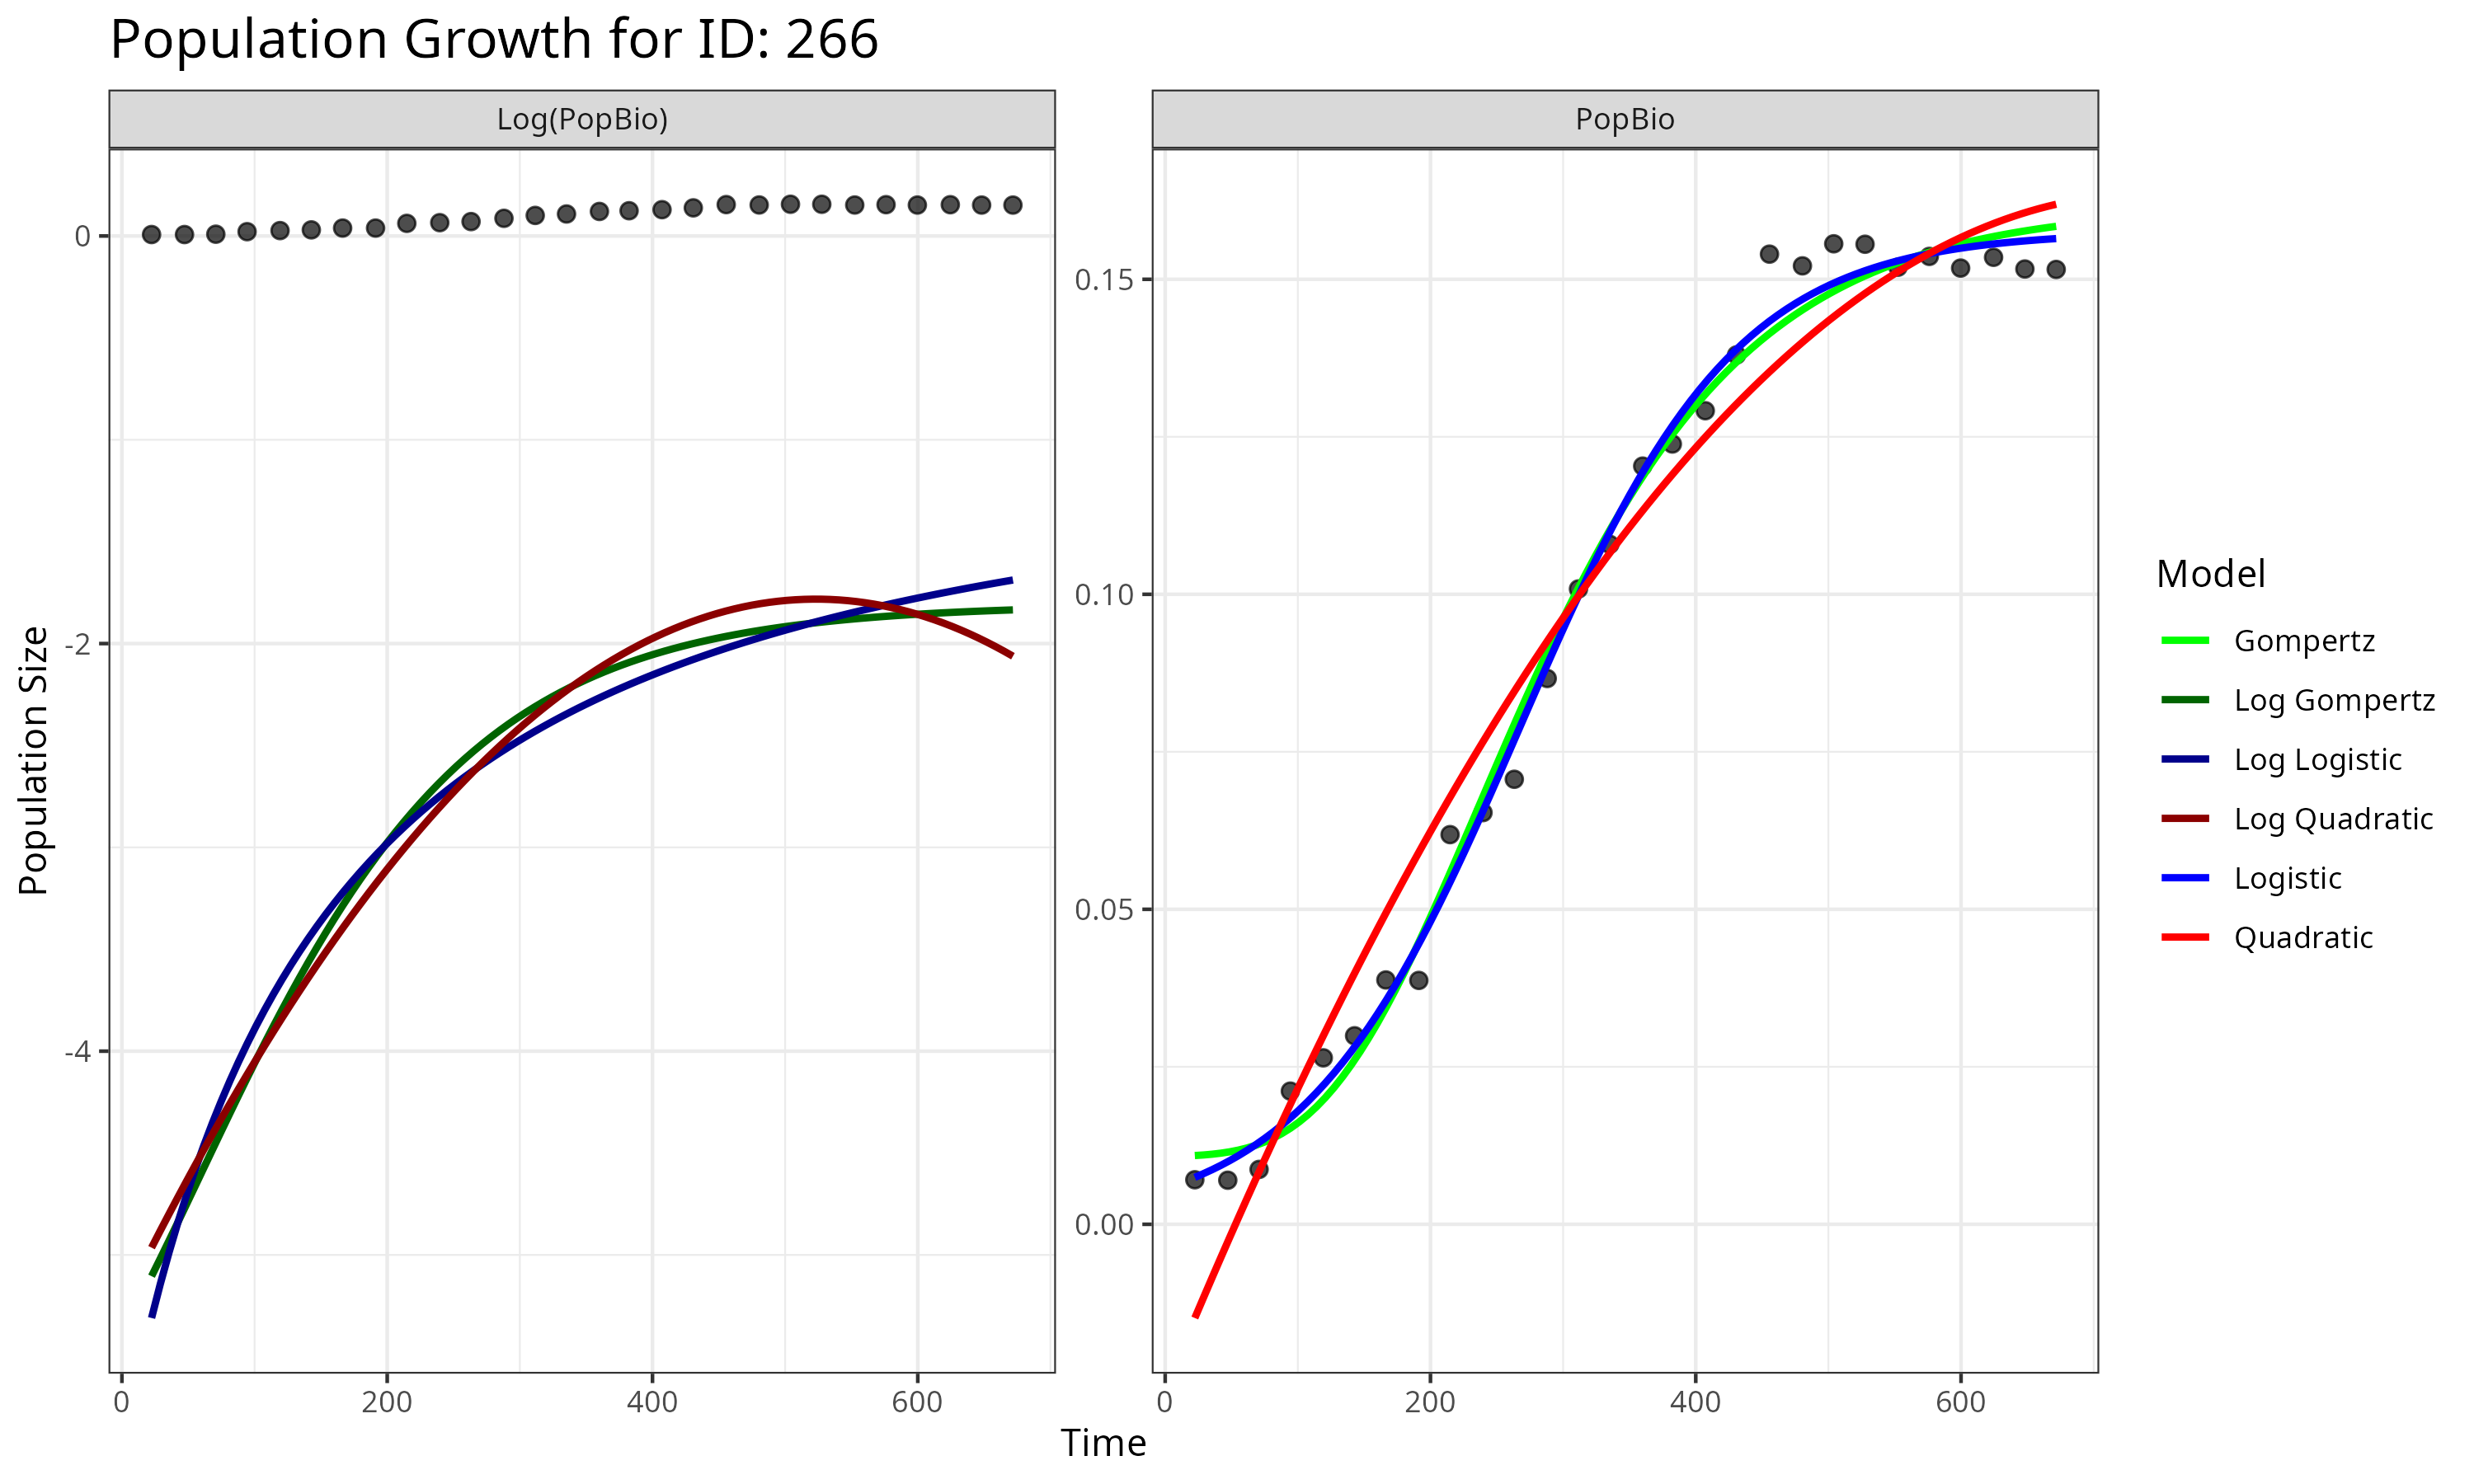
\includegraphics[width=0.8\linewidth]{../results/modelplots/Models_Comparison_plot_ID_266.png}
        \caption{Comparison of Quadratic, Logistic, Gompertz with log-transformed population size (left panel) and untransformed population size (right panel) for ID 266. The black dots represent observed population growth over time. The Gompertz (green) and Quadratic (red) models effectively represent both the growth phase and the stationary phase. The Log-Gompertz model (green) also provides a good fit but deviates slightly during the initial stages of growth. Dataset from \parencite[]{1Bae2014}}
    \label{fig:plot}
\end{figure}


\section*{Discussion}

Accurate mathematical models are essential for analysing and predicting bacterial population growth dynamics. Given the diverse growth patterns observed across various species, media, and temperature conditions, the model that provided the best fit in this study can be considered to demonstrate broad applicability for modelling microbial growth \parencite[]{Lopez2004}. 
Because bacterial growth data can be measured in various ways (OD, CFU, Dry Weight), selecting an appropriate model requires careful consideration of both measurement reliability and statistical properties. Due to heteroscedasticity in CFU and OD measurements, logarithmic transformation is commonly applied  \parencite[]{Lopez2004, SCHAFFNER1998185}. I therefore evaluated three models: Quadratic, Logistic, Gompertz models, in both log-transformed and not-transformed Population data. 

My findings align with \cite[]{Gibson1988}’s approach, as the Gompertz and Logistic models capture microbial growth dynamics with a "reasonable good-ness of fit". In my statistical analysis, the log Gompertz model emerged as the best-fitting model, consistently outperforming others in three out of four statistical criteria, including R². The log Logistic model had the lowest AICc, which was expected due to it having less parameters (compared to the Gompertz model). These results reinforce the suitability of the Gompertz model for describing microbial growth, particularly when applied to log-transformed data. This is likely because the Gompertz model captures the dynamic nature of growth, where the rate initially increases, reaches a peak, and then declines \parencite[]{Gibson1988, Jason1983}. However, \autoref{fig:plot} suggests that statistical fit does not always align with biological interpretability. In the left panel (log-transformed data), model predictions deviate more from observed values, whereas in the right panel (untransformed data), the curves align more closely with actual bacterial growth trends. The Gompertz and Logistic models (green and blue lines) effectively describe both the exponential and stationary phases, reinforcing their relevance in biological contexts.

The choice of model ultimately depends on the objective. For predictive accuracy, the log Gompertz model is optimal, as it explains the greatest variance (highest R²) and performs well across multiple statistical measures. Alternatively, the log Logistic model provides strong predictive performance with lower AICc, indicating a balance between fit and complexity. This may be due to the model's symmetry, as it assumes identical acceleration and deceleration of growth rate, which may not always be biologically accurate \parencite[]{Gibson1988}.

However, for biological realism, the untransformed Gompertz model is preferable, as it explicitly incorporates the lag phase (tlag), a key feature for describing bacterial growth dynamics. If both predictive accuracy and biological interpretability are needed, a phase-specific modelling approach, where different models are applied to distinct growth phases may provide the most comprehensive framework.
These results further highlight the need to evaluate growth models not only based on statistical criteria but also how well they align with observed growth patterns. Both statistically and visually, my analysis agrees that the Quadratic model did not directly incorporate biologically meaningful growth parameters and can lead to unrealistic predictions \parencite[]{Gibson1988}. Most of the models I considered fail to account for the bacterial population decline, commonly referred to as the death phase. My study also did not focus on this phase due to the lack of available data, as most datasets I used do not include population measurements during this stage. The exclusion is likely driven by time constraints, financial limitations, and a primary research focus on earlier growth phases, which are particularly relevant in microbiology and antibiotic treatment strategies. The initial growth stage, known as the lag phase, is when microorganisms adjust to their environment and gradually increase their growth potential \parencite{Kumakura2023}. A deeper understanding of the mechanisms that enable rapid acclimatisation could facilitate culturing microbes under optimal conditions \parencite{Rolfe2012}. Despite its importance to various industries, the lag phase remains the least understood phase of microbial growth due to the scarcity of available data \parencite[]{Rolfe2012}. 

Furthermore, the datasets analysed encompassed a range of biological and environmental conditions, including variations in growth media, temperature, and microbial species. As a result, model performance is likely to be influenced by these factors. Even when environmental conditions are controlled, genetic variability within bacterial populations can still lead to substantial differences in growth dynamics \parencite{Ackermann2015}. To enhance predictive accuracy, future research should incorporate these biological and environmental variables directly into model frameworks. However, due to the inherent complexity of bacterial growth, no single model is likely to capture all growth phases under all conditions. A more effective approach may involve phase-specific modelling, where distinct models are tailored to the lag, exponential, stationary, and death phases individually. This strategy could provide a more precise and biologically relevant representation of microbial growth patterns.

Overall, My study underscores the need for a balance between model complexity and practical applicability. While complex models may offer greater accuracy, they must remain interpretable and adaptable to real-world applications. By refining bacterial growth models with phase-specific insights and tailored biological parameters, future research can enhance predictive capabilities, leading to better antimicrobial strategies, biotechnological applications, and ecological modelling of microbial populations.





\newpage
\begin{sloppy}
\printbibliography
\end{sloppy}
\end{document}








